\documentclass{beamer}

\usepackage[utf8]{inputenc}
\usepackage[T1]{fontenc}
\usepackage[english,brazil]{babel}


% usando tema personalizado. 
% arquivo beamerthemeIFSC.sty deve estar no mesmo diretório do .tex
\usepackage{beamerthemeIFSC}

\usepackage[font=tiny]{caption} 


\title{Lei de Gauss — Elétrica}
\subtitle{Explorando a Lei de Gauss: Fundamentos, Aplicações e Relações com Ondas Eletromagnéticas}
\author{André Ghisleni Raimann}
\institute{Instituto Federal de Santa Catarina — Campus Chapecó}
\date{\today}

\begin{document}

  \begin{frame}
  \titlepage
  \end{frame}
  \section{Lei de Gauss Elétrica}
  \section{Lei de Gauss Elétrica}

  \begin{frame}{Enunciado}
  \begin{block}{Lei de Gauss}
  A Lei de Gauss é uma alternativa à Lei de Coulomb e afirma que o fluxo elétrico total através de uma superfície fechada é proporcional à carga elétrica total (líquida) existente no interior dessa superfície. 
  \end{block}
  
  % Imagem sugerida: Representação de uma carga puntiforme dentro de uma superfície fechada, com linhas de campo elétrico irradiando da carga.
  \begin{minipage}{0.5\textwidth}
    \centering
    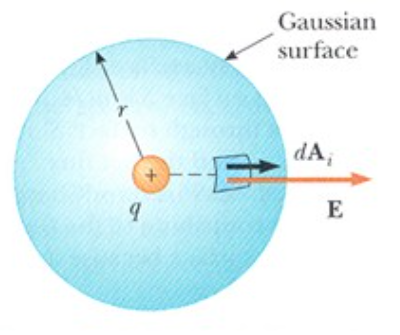
\includegraphics[width=0.5\textwidth]{images/lei_de_gauss.png}
  \end{minipage}%
  \hfill
  \begin{minipage}{0.45\textwidth}
    \begin{block}{Expressão Matemática}
    \[
    \Phi_E = \oint_S \mathbf{E} \cdot d\mathbf{A} = \frac{Q_{\text{int}}}{\epsilon_0}
    \]
    \end{block}
  \end{minipage}

  \end{frame}

  \section{Fluxo Magnético}

  \begin{frame}{Fluxo Magnético}
    \begin{block}{Definição}
    O fluxo magnético é uma medida da quantidade de campo magnético que atravessa uma superfície. É análogo ao conceito de fluxo elétrico na Lei de Gauss para campos elétricos. O fluxo magnético é representado pela integral do campo magnético através de uma superfície.
    \end{block}
    \begin{block}{Expressão Matemática}
      \[
      \Phi_B = \oint_S \mathbf{B} \cdot d\mathbf{A}
      \]
    \end{block}
    onde:
    \begin{itemize}
        \item $\Phi_B$ é o fluxo magnético.
        \item $\mathbf{B}$ é o vetor campo magnético.
        \item $d\mathbf{A}$ é o vetor área da superfície infinitesimal.
    \end{itemize}
  \end{frame}

  \begin{frame}{Fluxo Magnético}    
    \begin{block}{Lei de Gauss para o Magnetismo}
    A Lei de Gauss para o magnetismo afirma que o fluxo magnético total através de uma superfície fechada é zero, o que implica que não existem monopólos magnéticos:
    \[
    \oint_S \mathbf{B} \cdot d\mathbf{A} = 0
    \]
    \end{block}
    
    % Imagem sugerida: Representação gráfica do fluxo magnético através de uma superfície com linhas de campo magnético.
    % \begin{figure}
    % \centering
    % \includegraphics[width=0.8\textwidth]{path_to_image/fluxo_magnetico.png}
    % \caption{Fluxo magnético através de uma superfície}
    % \end{figure}
  \end{frame}
  
  \section{Importância e Aplicações}
  
  \begin{frame}{Importância e Aplicações}
  \begin{itemize}
      \item \textbf{Simplicidade em cálculos:} Permite o cálculo de campos elétricos em casos de alta simetria de forma direta.
      \item \textbf{Relação com as equações de Maxwell:} É uma das quatro equações de Maxwell que descrevem as leis fundamentais do eletromagnetismo.
      \item \textbf{Aplicações práticas:} Utilizada em dispositivos como capacitores, cabos coaxiais e sistemas de blindagem eletrostática.
  \end{itemize}
  
  % Imagem sugerida: Diagrama que mostra a aplicação da Lei de Gauss em diferentes configurações, como esferas, cilindros e planos.
  \begin{figure}
  \centering
  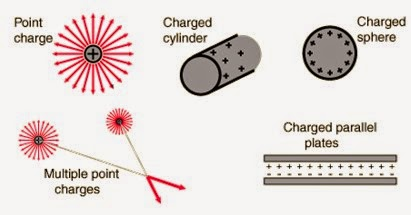
\includegraphics[width=0.4\textwidth]{images/aplicacoes_gauss.png}
  \caption{Aplicações da Lei de Gauss em diferentes simetrias}
  \end{figure}
  
  \end{frame}
  
  \section{Curiosidades e Explicações}
  
  \begin{frame}{Curiosidades}
  \begin{itemize}
      \item \textbf{Blindagem eletrostática:} A Lei de Gauss explica o funcionamento da blindagem eletrostática, onde uma carga externa não influencia o campo elétrico dentro de um condutor fechado.
      \item \textbf{Gaiola de Faraday:} Baseado na Lei de Gauss, a Gaiola de Faraday protege seu interior contra campos elétricos externos.
      \item \textbf{Cabos coaxiais:} Utilizados em transmissão de sinais, os cabos coaxiais usam o princípio da blindagem eletrostática para evitar interferência.
  \end{itemize}
  
  % Imagem sugerida: Ilustração de uma Gaiola de Faraday, mostrando como ela protege contra campos elétricos externos.
  \begin{figure}
  \centering
  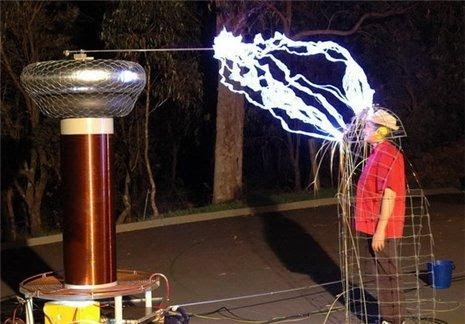
\includegraphics[width=0.3\textwidth]{images/gaiola_faraday.png}
  \caption{Ilustração de uma Gaiola de Faraday}
  \end{figure}
  
  \end{frame}
  
  \section{Formas Matemáticas}
  
  \begin{frame}{Formas Integral e Diferencial}
  \begin{block}{Forma Integral}
  \[
  \oint_S \mathbf{E} \cdot d\mathbf{A} = \frac{Q_{\text{int}}}{\epsilon_0}
  \]
  \end{block}
  
  \begin{block}{Forma Diferencial}
  \[
  \nabla \cdot \mathbf{E} = \frac{\rho}{\epsilon_0}
  \]
  \end{block}
  
  \end{frame}
  
  \section{Relação com as Ondas Eletromagnéticas}
  
  \begin{frame}{Equações de Maxwell e Ondas Eletromagnéticas}
  \begin{block}{Ondas Eletromagnéticas}
  As equações de Maxwell, incluindo a Lei de Gauss, descrevem como campos elétricos e magnéticos se comportam e se propagam no espaço. Uma solução importante dessas equações é a existência de ondas eletromagnéticas, como a luz, que são oscilações dos campos elétrico e magnético que se propagam no espaço.
  \end{block}
  
  % Imagem sugerida: Representação gráfica de uma onda eletromagnética propagando-se no espaço.
  \begin{figure}
  \centering
  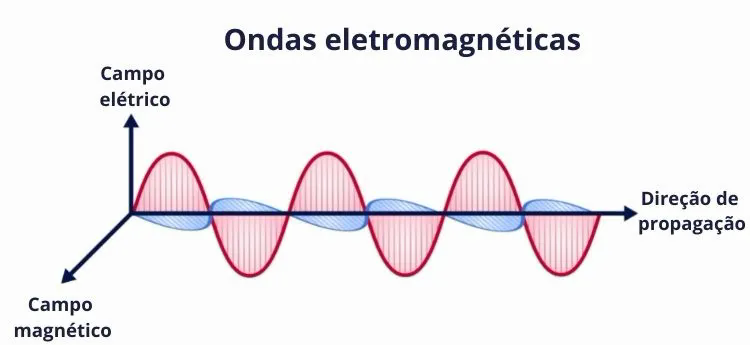
\includegraphics[width=0.5\textwidth]{images/onda_eletromagnetica.png}
  \caption{Propagação de uma onda eletromagnética}
  \end{figure}
  
  \end{frame}
  
  \section{Aplicações Práticas}
  
  \begin{frame}{Blindagem Eletrostática}
  \begin{block}{Definição}
  É a prática de isolar uma região do espaço de influências elétricas externas, usando condutores. A Lei de Gauss é fundamental para entender por que a carga em excesso em um condutor se distribui na superfície, deixando o interior livre de campos elétricos.
  \end{block}
  
  % Imagem sugerida: Demonstração de como a carga se distribui na superfície de um condutor oco.
  \begin{figure}
  \centering
  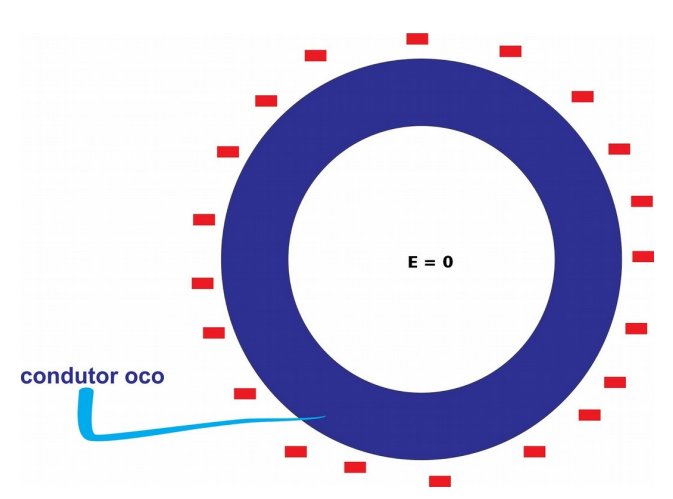
\includegraphics[width=0.4\textwidth]{images/blindagem_eletrostatica.png}
  \caption{Distribuição de carga em um condutor oco}
  \end{figure}
  
  \end{frame}
  
  \begin{frame}{Gaiola de Faraday}
  \begin{block}{Descrição}
  Uma Gaiola de Faraday é um exemplo de blindagem eletrostática, onde um condutor oco, como uma malha metálica, protege o interior de campos elétricos externos. É amplamente usada em laboratórios e na proteção de dispositivos eletrônicos.
  \end{block}
  
  % Imagem sugerida: Fotografia de uma Gaiola de Faraday em um experimento de laboratório.
  \begin{figure}
  \centering
  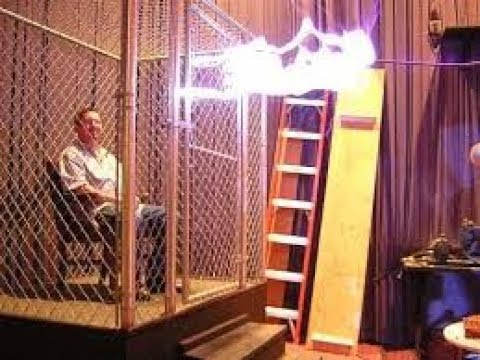
\includegraphics[width=0.4\textwidth]{images/gaiola_faraday_experimento.png}
  \caption{Gaiola de Faraday em um experimento de laboratório}
  \end{figure}
  
  \end{frame}
  
  \begin{frame}{Cabos Coaxiais}
  \begin{block}{Estrutura}
  Os cabos coaxiais utilizam o princípio da blindagem eletrostática para transmitir sinais elétricos com mínima interferência. Eles consistem em um condutor interno, isolado por um dielétrico, e cercado por uma blindagem condutora externa.
  \end{block}
  
  % Imagem sugerida: Corte transversal de um cabo coaxial, mostrando suas camadas internas.
  \begin{figure}
  \centering
  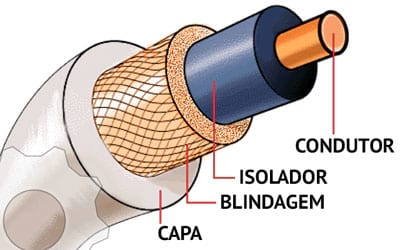
\includegraphics[width=0.5\textwidth]{images/cabo_coaxial.png}
  \caption{Corte transversal de um cabo coaxial}
  \end{figure}
  
  \end{frame}
  
  \begin{frame}{Veículos e Aviões}
  \begin{block}{Proteção}
  A estrutura metálica de veículos e aviões age como uma Gaiola de Faraday, protegendo os ocupantes de descargas elétricas, como raios.
  \end{block}
  
  % Imagem sugerida: Ilustração de um avião sendo atingido por um raio, mostrando a distribuição da corrente pelo exterior.
  \begin{figure}
  \centering
  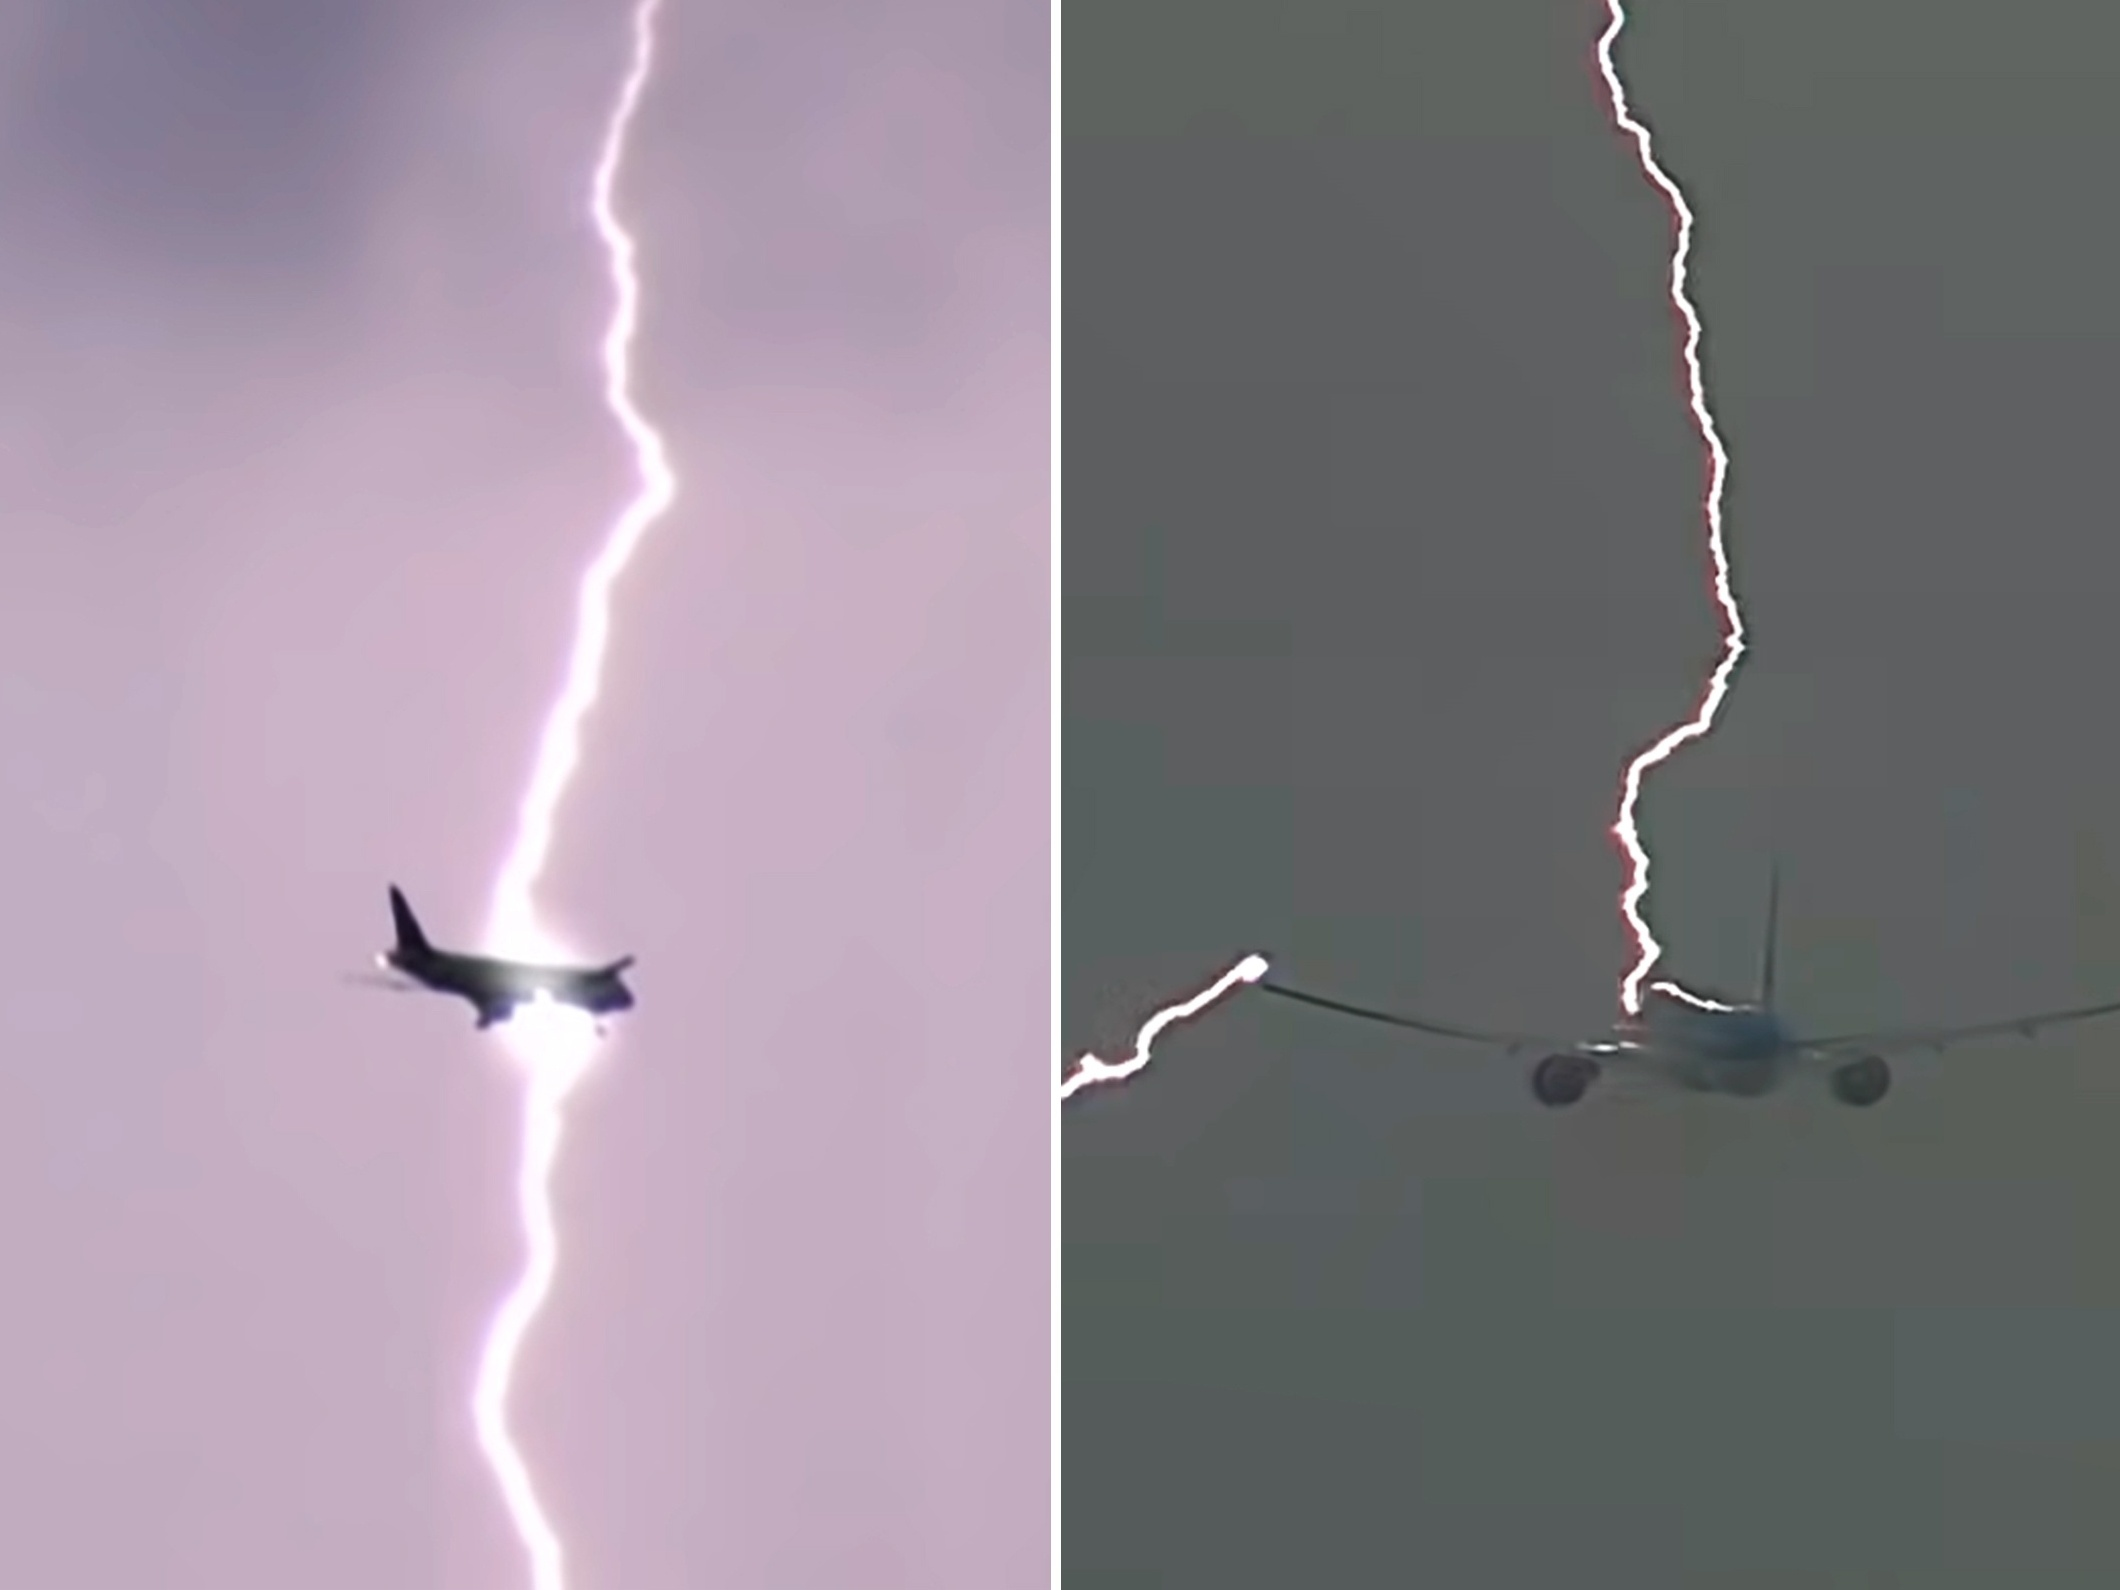
\includegraphics[width=0.4\textwidth]{images/aviao_raio.png}
  \caption{Distribuição de corrente em um avião atingido por um raio}
  \end{figure}
  
  \end{frame}
  
  \section{Simetrias no Campo Elétrico}
  
  \begin{frame}{Campo Elétrico em Simetrias}
  \begin{block}{Aplicação da Lei de Gauss}
  A Lei de Gauss é particularmente útil para descrever campos elétricos em configurações com simetria esférica, cilíndrica e planar, onde o cálculo direto da distribuição do campo elétrico é simplificado.
  \end{block}
  
  % Imagem sugerida: Diagrama que ilustra o campo elétrico em torno de uma carga em uma configuração esférica, cilíndrica e planar.
  % \begin{figure}
  % \centering
  % \includegraphics[width=0.8\textwidth]{images/simetria_campo_eletrico.png}
  % \caption{Campo elétrico em diferentes simetrias}
  % \end{figure}
  
  \end{frame}

  \begin{frame}{Cálculo do Campo Elétrico via Lei de Gauss}

    \begin{itemize}
      \item Assumindo uma superfície gaussiana esférica centrada em $Q$ e de raio $r$, o campo $E$ é igual em todos os pontos da superfície.
    \end{itemize}

    \center 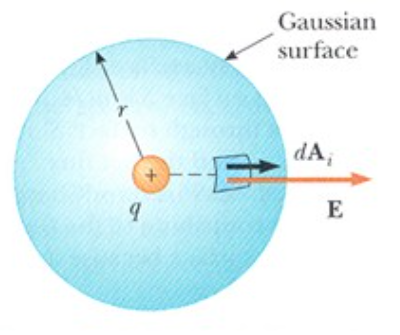
\includegraphics[width=0.2\textwidth]{images/lei_de_gauss.png}

    $\Phi = \oint \mathbf{E} \cdot d\mathbf{A} = \frac{Q}{\epsilon_0} \qquad \implies \qquad E \oint d\mathbf{A} = \frac{Q}{\epsilon_0} \qquad \implies \qquad E \cdot A = \frac{Q}{\epsilon_0}$

    \begin{itemize}
      \item A área total da esfera é $A = 4\pi r^2$. Assim sendo:
    \end{itemize}
      
    \[ E \cdot 4 \pi r^2 = \frac{Q}{\epsilon_0} \qquad \implies \qquad E = \frac{1}{4 \pi \epsilon_0} \frac{Q}{r^2} \]
    
  \end{frame}
  
  

\end{document}